\section{Experimental Procedure and Hypotheses}
\label{sec:experimental_procedure}

The experimental procedure is designed to evaluate how selected configuration variables affect the performance and cost behaviour of the modular ZK-rollup benchmarking framework. Each experiment changes one primary configuration dimension while keeping the workload model, local Layer-1 environment, and measurement pipeline consistent. This supports fair comparison across configurations and reduces the influence of external factors such as public-network congestion or fluctuating gas prices.

Figure~\ref{fig:experiment_pipeline} summarizes the experimental benchmarking pipeline. The process begins with a selected benchmark configuration, followed by environment initialization, workload generation, telemetry collection, metric aggregation, and cross-configuration analysis.

\begin{figure}[!htbp]
    \centering
    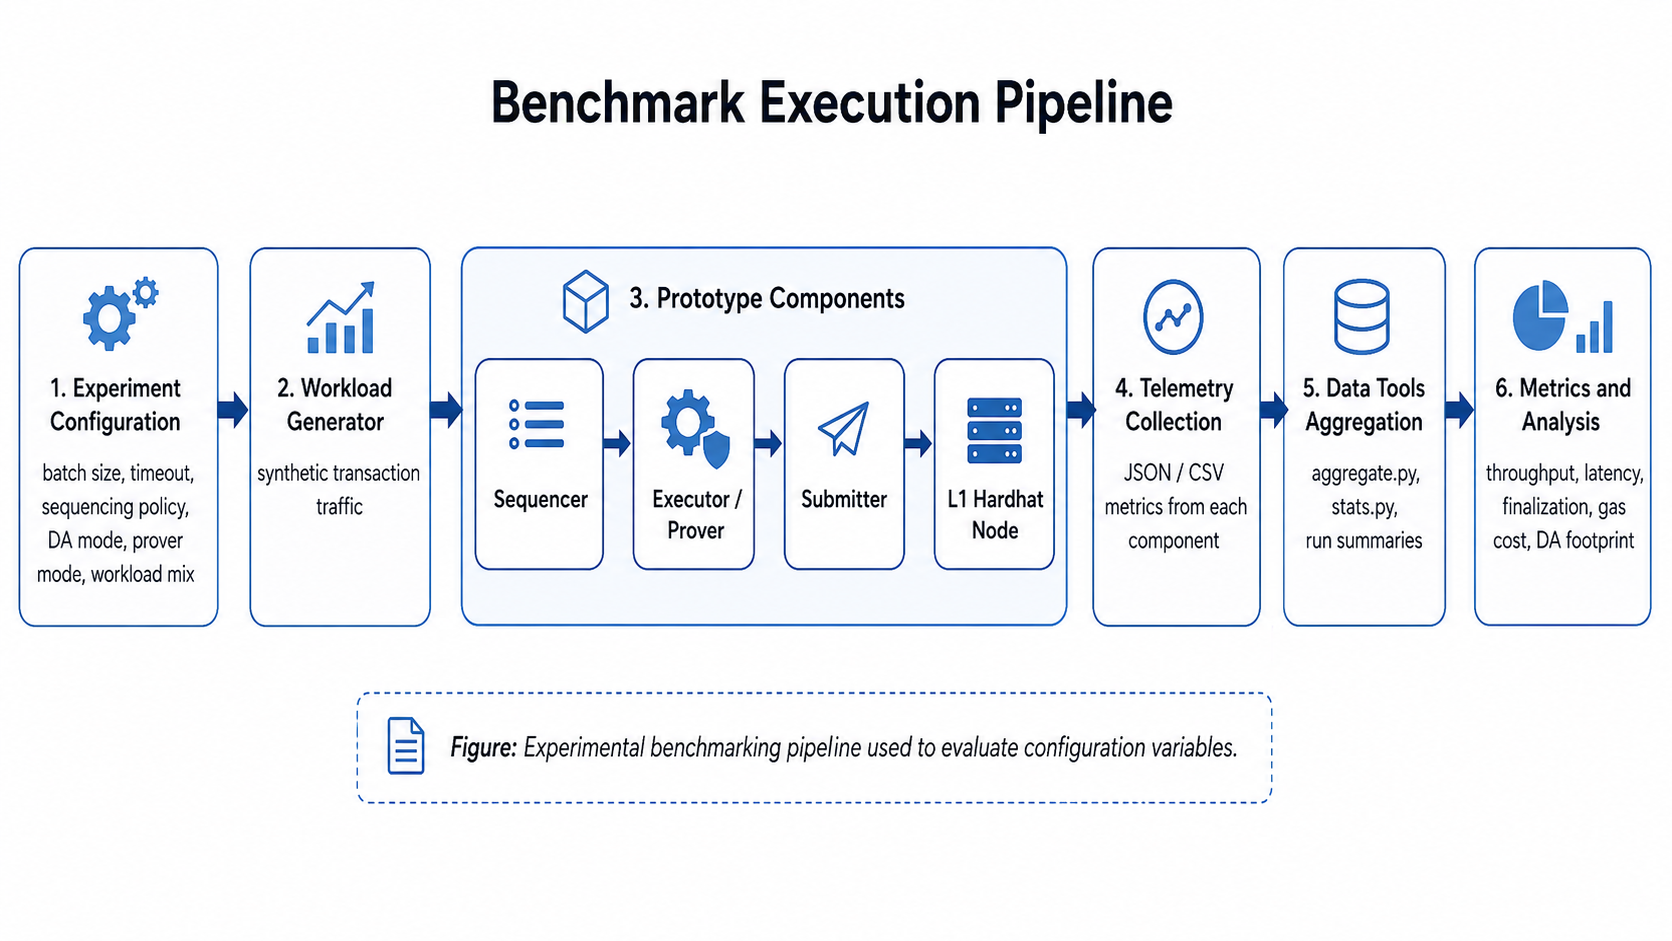
\includegraphics[width=0.95\textwidth]{./figures/pipeline.png}
    \caption{Experimental benchmarking pipeline used to evaluate configuration variables.}
    \label{fig:experiment_pipeline}
\end{figure}

Experiments are conducted by systematically sweeping configuration variables using bash orchestration scripts. For each run, the benchmark stack is started with a selected configuration, synthetic traffic is generated using the workload generator, and raw telemetry is collected from the Sequencer, Executor, Submitter, and workload tools. The Data Tools pipeline then aggregates these raw JSON, JSONL, and CSV outputs into final performance and cost metrics.

The experimental procedure follows six main steps:

\begin{enumerate}
    \item \textbf{Configuration selection:}
    A benchmark configuration is selected by setting variables such as \path{max_batch_size}, \path{timeout_interval_ms}, \path{sequencing_policy}, \path{prover_backend}, \path{mock_proof_delay}, and \path{da_mode}.

    \item \textbf{Environment initialization:}
    The local rollup environment is started using Docker-based orchestration. The Layer-1 settlement layer runs on a local Hardhat node to remove public-network variability.

    \item \textbf{Workload execution:}
    The Python workload generator submits synthetic transactions using the configured transaction rate, duration, seed, transaction mix, concurrency level, and burst settings.

    \item \textbf{Telemetry collection:}
    During the run, each component writes raw metrics to the benchmark metrics directory. These metrics capture queueing, batching, execution, proving, data availability formatting, Layer-1 submission, and cost-related behaviour.

    \item \textbf{Metric aggregation:}
    Python aggregation scripts process the collected telemetry and compute run-level metrics such as throughput, latency percentiles, proof time, finalization time, data availability footprint, gas usage, and cost per transaction.

    \item \textbf{Cross-configuration comparison:}
    The aggregated metrics are compared across benchmark runs to identify bottlenecks and trade-offs between throughput, latency, finality, proving overhead, and data availability cost.
\end{enumerate}

The benchmark plan is guided by the hypotheses shown in Table~\ref{tab:experimental_hypotheses}. These hypotheses are derived from the expected behaviour of rollup systems, where batching improves cost amortization, data availability mode affects Layer-1 footprint, and proving delay can dominate the execution pipeline.

\begin{table}[!htbp]
\centering
\caption{Experimental Hypotheses and Expected Observations}
\label{tab:experimental_hypotheses}
\compacttable
\begin{tabularx}{\textwidth}{@{}p{0.22\textwidth}Y Y@{}}
\toprule
\textbf{Experiment} & \textbf{Hypothesis} & \textbf{Main metrics observed} \\
\midrule

Batch size sweep
& Larger batches are expected to reduce amortized cost per transaction, but increase average waiting time and soft-finality latency.
& Batch size, throughput, average latency, P95 latency, cost per transaction, and Layer-1 gas per transaction. \\

\addlinespace

Data availability mode comparison
& Blob-based submission is expected to reduce the data availability gas footprint compared with calldata, especially for larger or DA-heavy batches.
& Data availability bytes, compressed bytes, blob utilization, Layer-1 gas used, and cost per transaction. \\

\addlinespace

Mock proof delay sweep
& Increasing the simulated proof delay is expected to shift the bottleneck from Layer-1 submission toward the Executor/Prover stage.
& Proof time, Executor delay, goodput TPS, batch finalization time, and tail latency. \\

\addlinespace

Sequencing policy comparison
& Different sequencing policies are expected to affect latency distribution and ordering behaviour, particularly under high-load conditions.
& Average latency, P95/P99 latency, per-class latency, success rate, and batch composition. \\

\addlinespace

Burst-load experiment
& Temporary burst traffic is expected to create queue buildup. Adaptive batching may improve recovery, but latency spikes can still occur when input load exceeds processing capacity.
& Queue depth, sealing reason, goodput TPS, P95/P99 latency, and recovery time after burst. \\

\bottomrule
\end{tabularx}
\end{table}
\normalsize

The batch size sweep directly evaluates the trade-off between economic efficiency and user-facing latency. Larger batches are expected to reduce the fixed Layer-1 and proof-verification cost per transaction because these costs are shared across more transactions. However, larger target batch sizes can also increase queueing delay because transactions may wait longer before the batch is sealed.

The data availability comparison evaluates the difference between calldata and EIP-4844 blob-style submission. Calldata provides a simple Ethereum-anchored data availability path, but it can become expensive as payload size increases. Blob-based submission is expected to reduce the cost of publishing larger payloads by using the blob data path, although the measured effect depends on whether the benchmark run uses real blob gas measurements or estimated blob gas values.

The mock proof delay sweep isolates the effect of proof-generation overhead. When proof delay is small, the bottleneck may remain in batching, submission, or Layer-1 settlement. As the configured proof delay increases, the Executor/Prover stage is expected to dominate the pipeline, increasing finalization time and reducing effective throughput.

Finally, sequencing and burst-load experiments evaluate system behaviour under changing traffic pressure. Policies such as FCFS, FeePriority, TimeBoost, FairBFT, and BlobPacking may produce similar average throughput under light load, but they can differ significantly in latency distribution, ordering fairness, and data availability efficiency under high-load or burst-load conditions.